\section{Experiments}
\label{sec:experiments}

\subsection{Baselines (Stage 1)}
\Cref{tab:baselines} reports the nine fine-tuned baselines. Seed variation is already comparable to the 0.5\,\pp tolerance on \dermamnist and \pneumnist, which is why every selection rule below is applied per seed rather than to the mean.

\begin{table}[t]
  \centering
  \small
  \begin{tabular}{lrrr}
    \toprule
    Dataset & Epochs & Val.\ acc.\ (\%) & Val.\ AUROC \\
    \midrule
    \pathmnist  & 5  & $99.85 \pm 0.03$ & 1.000 \\
    \dermamnist & 10 & $89.43 \pm 0.85$ & 0.983 \\
    \pneumnist  & 5  & $98.16 \pm 0.79$ & 0.999 \\
    \bottomrule
  \end{tabular}
  \caption{Full-parameter \deit baselines, mean $\pm$ SD over three training seeds. Validation only; test is untouched until \cref{sec:locked}.}
  \label{tab:baselines}
\end{table}

\subsection{Validation screen (Stage 2)}
\Cref{fig:screen} plots validation accuracy against retained tokens for all four methods, three seeds and, for random deletion, three masks (279 configurations). Applying the per-seed 0.5\,\pp rule gives very different budgets: \pathmnist tolerates merging down to 20 tokens (89.8\% reduction, 99.54\% vs.\ 99.85\%), \dermamnist tolerates only 147 tokens with EViT-style fusion (25\%), and \pneumnist 69 tokens with merging (64.8\%), where merging actually \emph{raised} mean validation accuracy to 98.73\%. Deletion of any kind failed to qualify on \pneumnist. At matched budgets attention ranking beat random deletion on \dermamnist but was worse on \pathmnist (99.04\% vs.\ 99.61\% at 49 tokens) and \pneumnist, so attention importance is not a safe default. EViT-style fusion was indistinguishable from plain attention deletion (e.g.\ 88.57\% vs.\ 88.60\% at 98 tokens on \dermamnist), whereas merging extended the tolerable budget substantially on two of three datasets.

\begin{figure}[t]
  \centering
  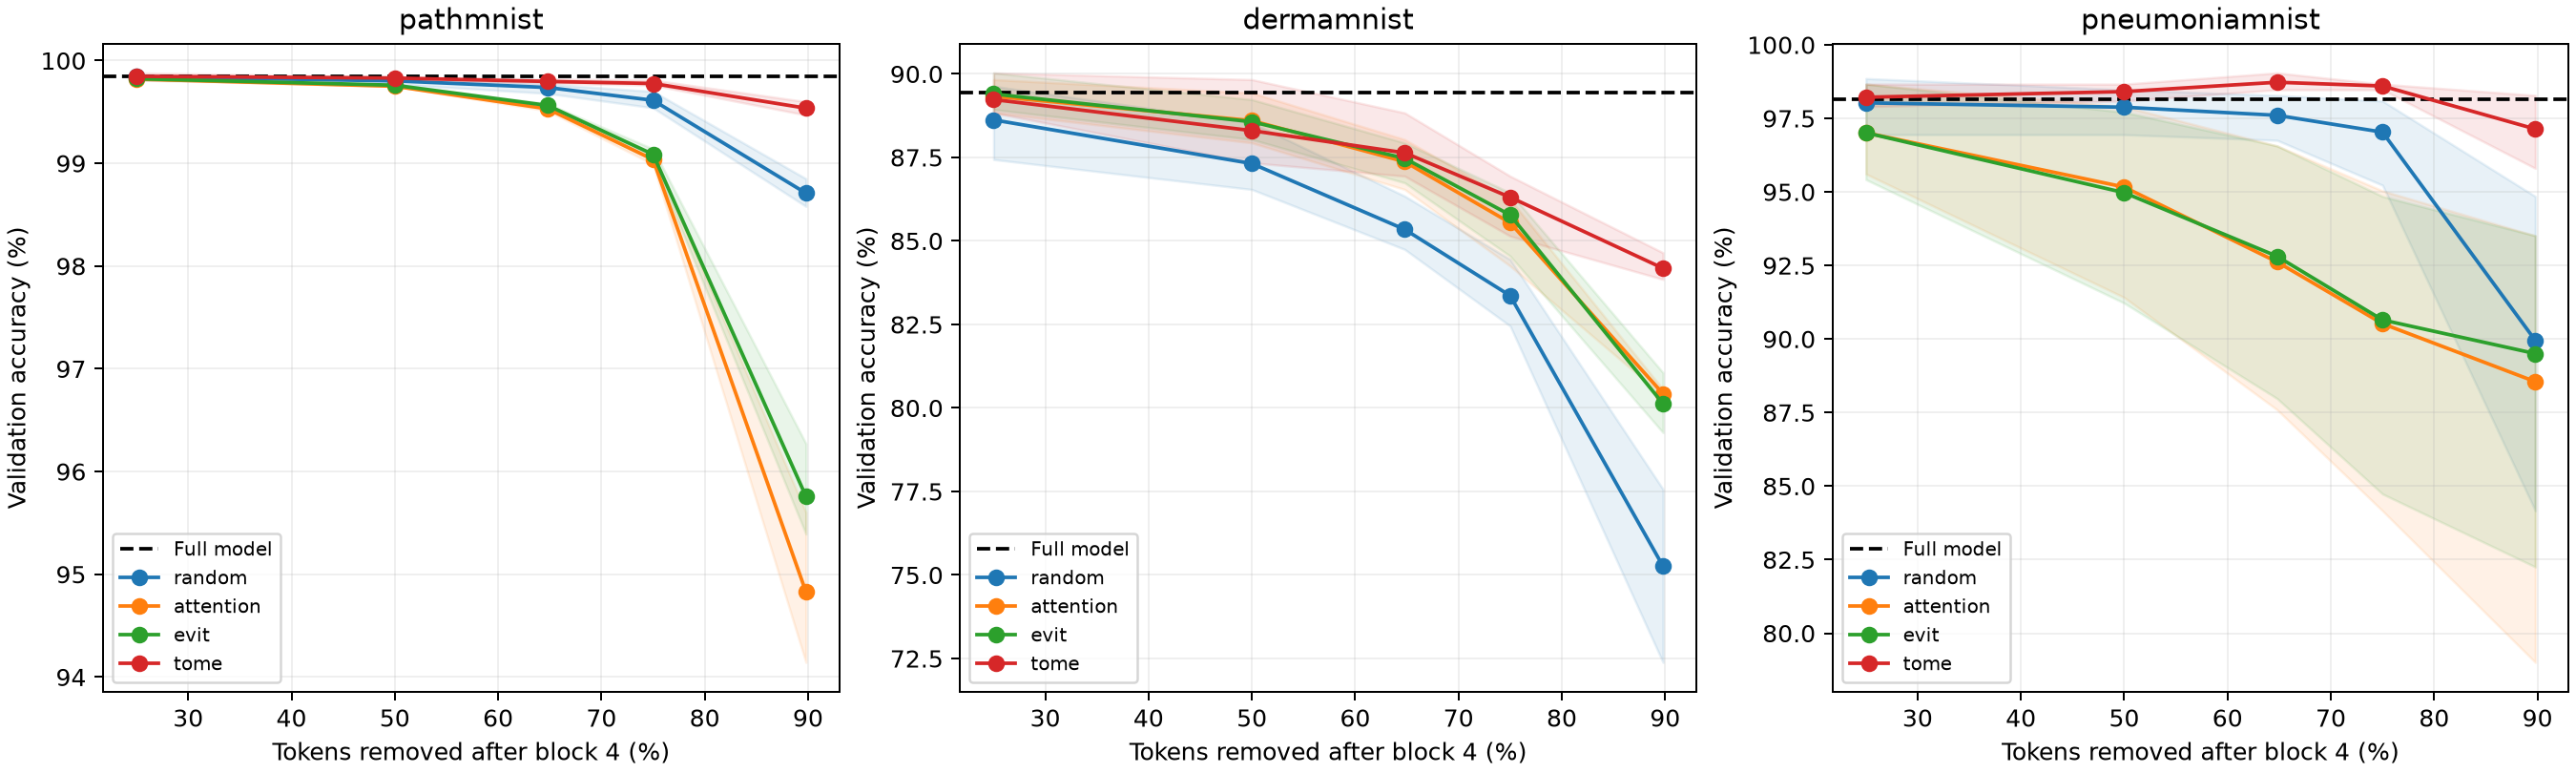
\includegraphics[width=\linewidth]{fig/accuracy_tradeoffs.png}
  \caption{Validation accuracy versus retained image tokens after block 4 for each dataset and method. Shading is the observed range across seeds and masks. Horizontal lines mark the full model and the 0.5\,\pp tolerance.}
  \label{fig:screen}
\end{figure}

\subsection{Ablations (Stage 3)}
\label{sec:ablations}
\textbf{Depth.} Merging \pathmnist to 20 tokens after block 1, 4 or 8 gives 70.4\%, 99.5\% and 99.9\% at 1.7, 3.8 and 6.5 GFLOPs (full model 9.2). The relationship is not monotonic: \pneumnist is better after block 4 (98.7\%) than block 8 (98.0\%). \textbf{Input removal} is far more damaging than intermediate reduction at the same count: keeping 20 of 196 \pathmnist patches before block 1 drops accuracy to 88.1\% (random) or 83.8\% (uniform grid), and 69 \pneumnist patches give 90.3\%. \textbf{Progressive} merging over blocks 4, 7 and 10 to 20 tokens on \pathmnist reaches 99.83\% at 4.81 GFLOPs versus 99.79\% for a single reduction to 56 tokens at 4.81 GFLOPs, but is slower at batch 1 (3.06 vs.\ 2.35\,ms), so it buys nothing on this hardware. \textbf{Recovery} (two epochs at the next-more-aggressive budget) recovers validation accuracy to within 0.1\,\pp of its matched control on all three datasets. \Cref{fig:examples} shows which patches attention deletion keeps.

\begin{figure}[t]
  \centering
  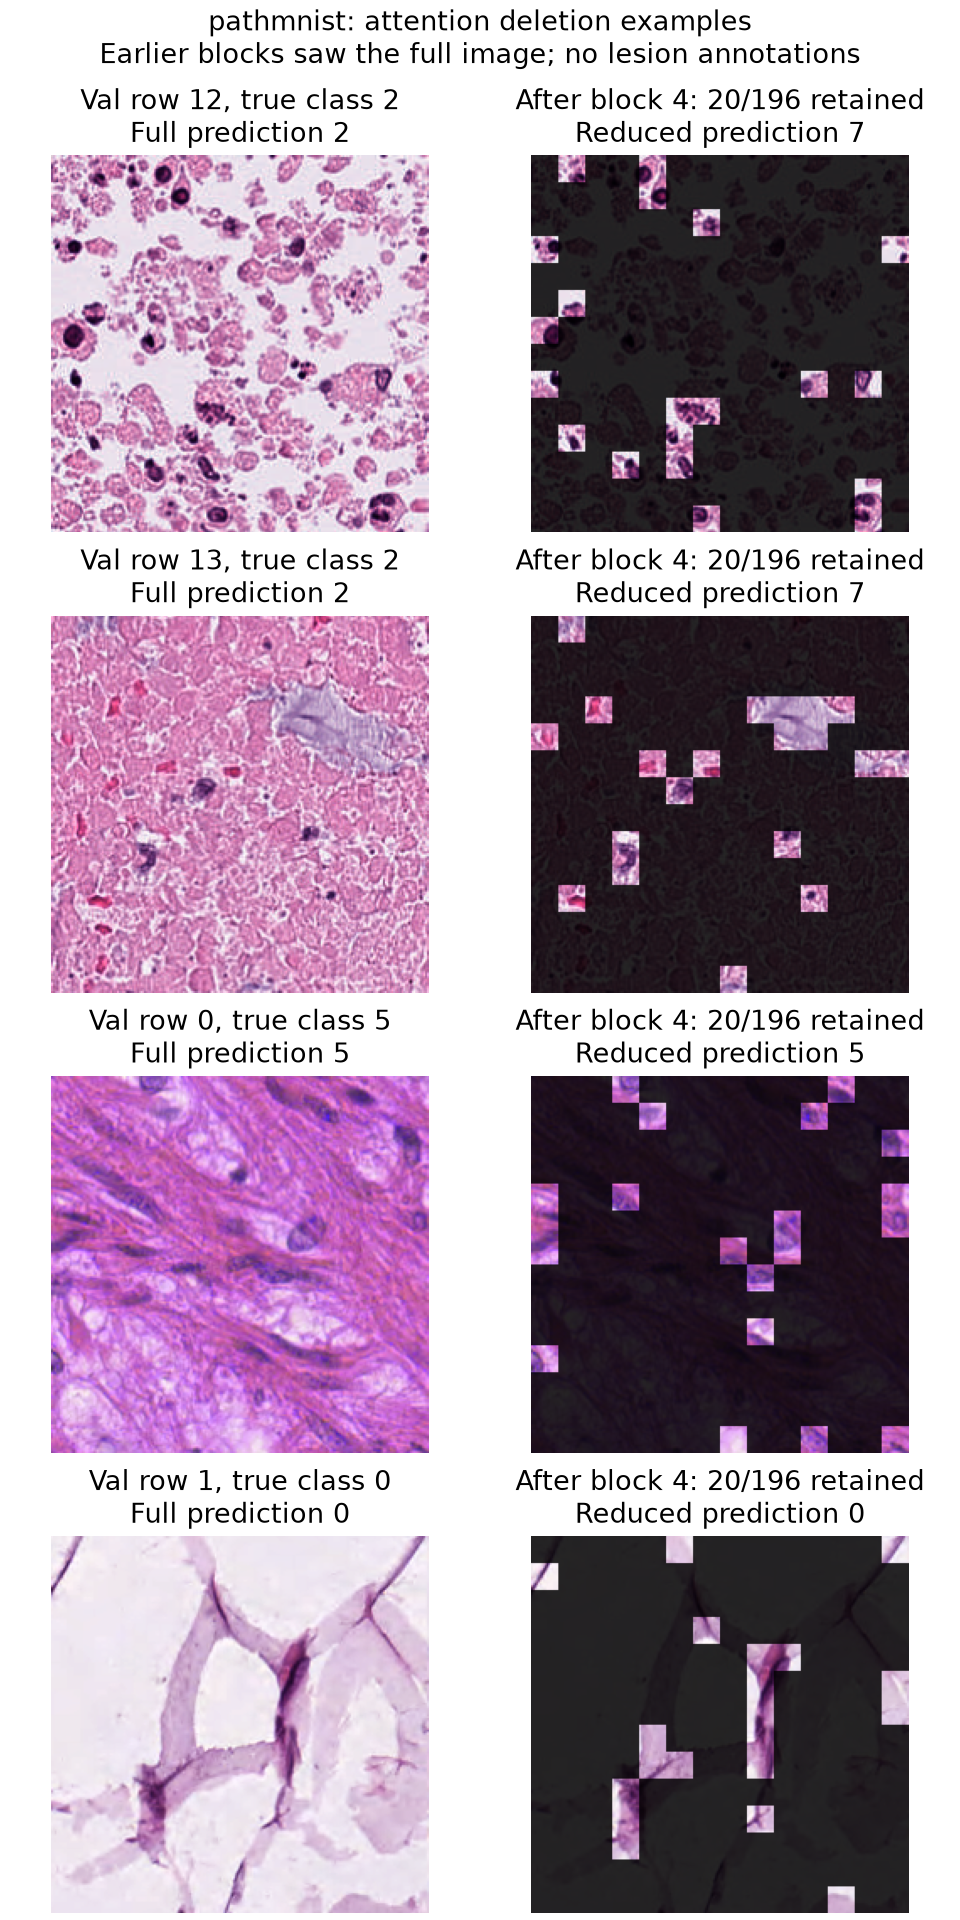
\includegraphics[width=\linewidth]{fig/pathmnist_examples.png}
  \caption{Attention deletion after block 4 on \pathmnist validation images; dimmed patches are removed from later blocks. Illustrative only: without region annotations these overlays cannot validate diagnostic localisation.}
  \label{fig:examples}
\end{figure}

\subsection{Locked test confirmation (Stage 4)}
\label{sec:locked}
\Cref{tab:test} is the main result. Every candidate is the validation winner for its method, frozen before test; recovery rows are paired with equally trained full-token controls. \Cref{fig:paired} shows the per-seed paired differences.

\begin{table*}[t]
  \centering
  \small
  \begin{tabular}{llrrrrrcc}
    \toprule
    Dataset & Policy & Tokens & Reduction & Ref.\ acc.\ & Reduced acc.\ & $\Delta$ mean & Worst LB & NI at 0.5 / 1\,\pp \\
    \midrule
    \pathmnist  & Attention, locked      & 69  & 64.8\% & 96.70 & 95.13 & $-1.57$ & $-2.44$ & no / no \\
    \pathmnist  & EViT-style, locked     & 69  & 64.8\% & 96.70 & 95.06 & $-1.64$ & $-2.59$ & no / no \\
    \pathmnist  & Random, locked         & 49  & 75.0\% & 96.70 & 94.98 & $-1.72$ & $-2.75$ & no / no \\
    \pathmnist  & ToMe-style, locked     & 20  & 89.8\% & 96.70 & 93.94 & $-2.77$ & $-4.28$ & no / no \\
    \pathmnist  & ToMe-style + recovery  & 20  & 89.8\% & 96.12 & 96.30 & $+0.18$ & $-1.12$ & no / no \\
    \midrule
    \dermamnist & Attention, locked      & 147 & 25.0\% & 90.57 & 90.27 & $-0.30$ & $-1.34$ & no / no \\
    \dermamnist & EViT-style, locked     & 147 & 25.0\% & 90.57 & 90.24 & $-0.33$ & $-1.43$ & no / no \\
    \dermamnist & EViT-style + recovery  & 98  & 50.0\% & 90.37 & 90.09 & $-0.28$ & $-1.93$ & no / no \\
    \midrule
    \pneumnist  & ToMe-style, locked     & 69  & 64.8\% & 95.03 & 93.27 & $-1.76$ & $-5.31$ & no / no \\
    \pneumnist  & ToMe-style + recovery  & 49  & 75.0\% & 95.62 & 95.30 & $-0.32$ & $-2.57$ & no / no \\
    \bottomrule
  \end{tabular}
  \caption{Locked test results. Accuracies (\%) and $\Delta$ (\pp) are means over three training seeds; ``Worst LB'' is the smallest conservative simultaneous 95\% lower bound on $\Delta$ among the seeds. Non-inferiority (NI) requires every seed's bound to exceed $-0.5$ (or $-1$)\,\pp. No candidate passed. \TODO{Verify the per-policy reduced accuracies against \texttt{reports/stage4/comparisons.json}; the reference/recovery columns are from the Stage 4 summary.}}
  \label{tab:test}
\end{table*}

\begin{figure}[t]
  \centering
  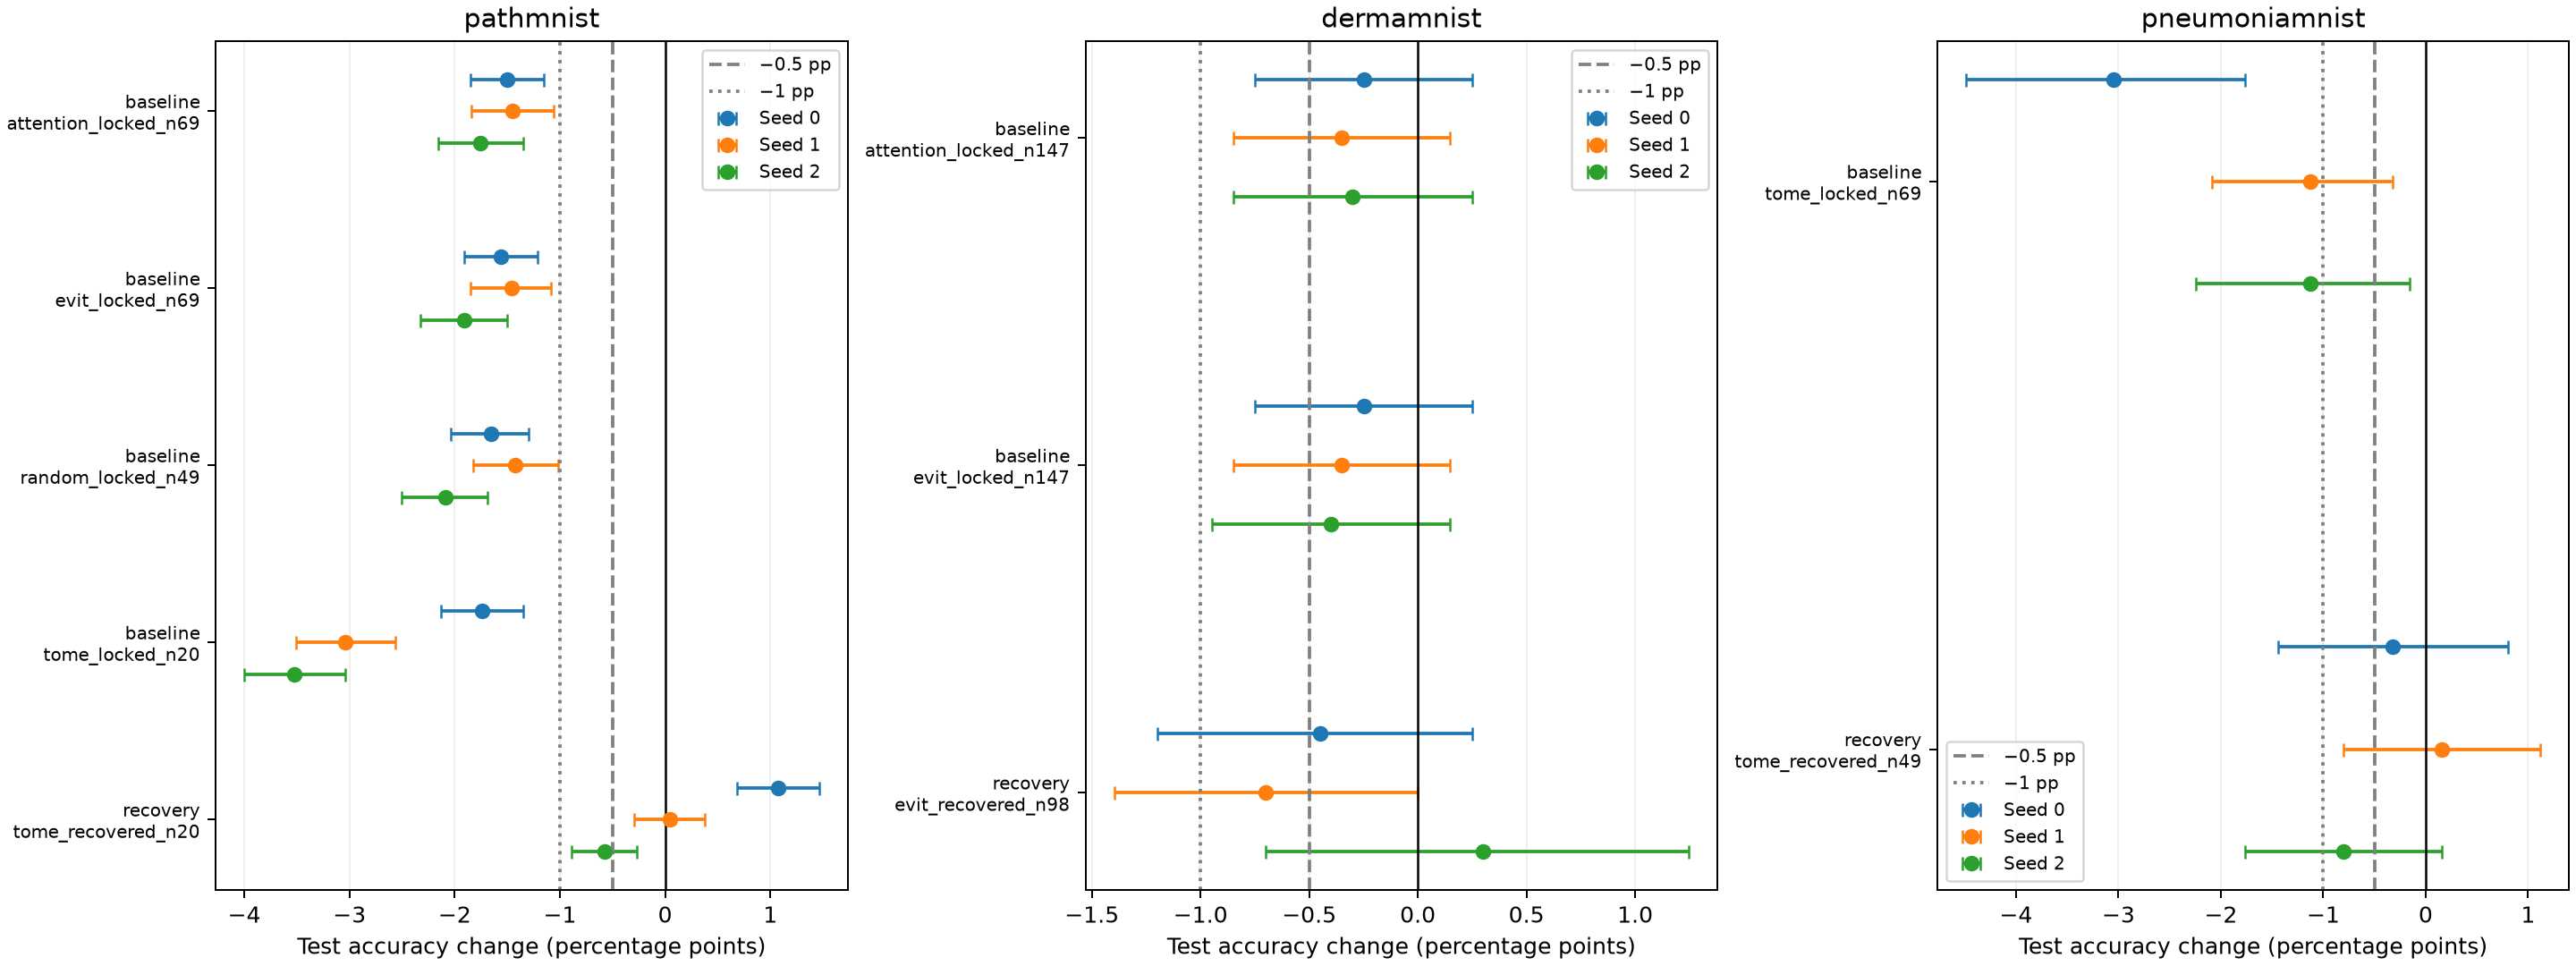
\includegraphics[width=\linewidth]{fig/paired_test_differences.png}
  \caption{Paired test accuracy differences (reduced minus reference) per seed with descriptive bootstrap 95\% intervals. Decisions in \cref{tab:test} use the more conservative simultaneous bounds.}
  \label{fig:paired}
\end{figure}

Three patterns stand out. First, \pathmnist's apparent robustness on validation did not transfer: all four locked policies lost 1.6--2.8\,\pp on a test set drawn from a different centre, and the 20-token merged model lost up to 12.4\,\pp of cancer-associated-stroma recall in one seed. Second, \dermamnist's conservative 147-token policies lost only 0.3\,\pp on average, but the 2{,}005-image test set yields bounds no tighter than $-1.3$\,\pp. Third, recovery helped everywhere, moving mean losses to $-0.3$\,\pp or better, yet seed-to-seed spread (e.g.\ $-0.57$ to $+1.07$\,\pp on \pathmnist) kept at least one bound below the margin in every case. None of the ten candidates established either margin.

\subsection{Compute and measured speed}
\Cref{tab:eff} shows that FLOP reduction and wall-clock gain diverge. Merging to 20 tokens cuts FLOPs by 59\% and raises batch-32 throughput by 75\%, but \emph{increases} batch-1 latency by 22\% because the matching step is not hidden at batch size 1. Only the mild \dermamnist fusion policy improves both. Any claim of ``$k\times$ faster'' for token reduction therefore needs to state the batch size.

\begin{table}[t]
  \centering
  \small
  \setlength{\tabcolsep}{4pt}
  \begin{tabular}{llrrr}
    \toprule
    Dataset & Policy & GFLOPs & Lat.\ (ms, b=1) & img/s (b=32) \\
    \midrule
    \pathmnist  & ToMe 20  & $9.20\!\to\!3.75$ & $2.13\!\to\!2.61$ & $3202\!\to\!5607$ \\
    \dermamnist & EViT 147 & $9.20\!\to\!7.66$ & $2.14\!\to\!2.01$ & $3171\!\to\!3614$ \\
    \pneumnist  & ToMe 69  & $9.20\!\to\!5.19$ & $2.15\!\to\!2.32$ & $3152\!\to\!4538$ \\
    \bottomrule
  \end{tabular}
  \caption{Full $\to$ reduced compute and speed on test inputs for the validation-selected policies without recovery (float32, means over three seeds, overhead of selection/merging included).}
  \label{tab:eff}
\end{table}

\subsection{Fine-tuning method comparison}
\label{sec:ftgrid}
\TODO{Fill from \texttt{outputs/finetune/*/*/seed\_*/training\_summary.json} (scripts/finetune\_grid.sh prints the table) and \texttt{outputs/pruning\_study/summary.md}.} We fine-tune each dataset with the four methods of \cref{sec:finetune} and three seeds (36 runs), then (a) sweep every checkpoint over the full Stage 2 budget grid on test, descriptively, to see whether the adaptation method changes pruning tolerance, and (b) compare full-parameter and LoRA recovery from the same starting checkpoint under the locked recovery budgets, each against its own equally trained control.

\begin{table}[t]
  \centering
  \small
  \setlength{\tabcolsep}{4pt}
  \begin{tabular}{llrrrr}
    \toprule
    Dataset & Method & Train.\ params & Val.\ acc.\ & Time (s) & Mem (GB) \\
    \midrule
    \multirow{4}{*}{\pathmnist}  & Full    & 21.7M & \TODO{} & \TODO{} & \TODO{} \\
                            & Partial & \TODO{} & \TODO{} & \TODO{} & \TODO{} \\
                            & LoRA    & \TODO{} & \TODO{} & \TODO{} & \TODO{} \\
                            & Linear  & \TODO{} & \TODO{} & \TODO{} & \TODO{} \\
    \midrule
    \multirow{4}{*}{\dermamnist} & Full    & \TODO{} & \TODO{} & \TODO{} & \TODO{} \\
                            & Partial & \TODO{} & \TODO{} & \TODO{} & \TODO{} \\
                            & LoRA    & \TODO{} & \TODO{} & \TODO{} & \TODO{} \\
                            & Linear  & \TODO{} & \TODO{} & \TODO{} & \TODO{} \\
    \midrule
    \multirow{4}{*}{\pneumnist}  & Full    & \TODO{} & \TODO{} & \TODO{} & \TODO{} \\
                            & Partial & \TODO{} & \TODO{} & \TODO{} & \TODO{} \\
                            & LoRA    & \TODO{} & \TODO{} & \TODO{} & \TODO{} \\
                            & Linear  & \TODO{} & \TODO{} & \TODO{} & \TODO{} \\
    \bottomrule
  \end{tabular}
  \caption{Adaptation methods: trainable parameters, best validation accuracy (mean over three seeds), optimisation-only training time and peak GPU memory. \TODO{Hardware for these runs.}}
  \label{tab:ftgrid}
\end{table}

\begin{table}[t]
  \centering
  \small
  \setlength{\tabcolsep}{4pt}
  \begin{tabular}{llrrr}
    \toprule
    Dataset & Recovery & Tokens & Test $\Delta$ vs.\ own control & Worst LB \\
    \midrule
    \pathmnist  & Full params       & 20 & \TODO{} & \TODO{} \\
    \pathmnist  & LoRA              & 20 & \TODO{} & \TODO{} \\
    \pathmnist  & LoRA from LoRA FT & 20 & \TODO{} & \TODO{} \\
    \dermamnist & Full params       & 98 & \TODO{} & \TODO{} \\
    \dermamnist & LoRA              & 98 & \TODO{} & \TODO{} \\
    \dermamnist & LoRA from LoRA FT & 98 & \TODO{} & \TODO{} \\
    \pneumnist  & Full params       & 49 & \TODO{} & \TODO{} \\
    \pneumnist  & LoRA              & 49 & \TODO{} & \TODO{} \\
    \pneumnist  & LoRA from LoRA FT & 49 & \TODO{} & \TODO{} \\
    \bottomrule
  \end{tabular}
  \caption{Recovery under the locked budgets with full-parameter versus LoRA-only updates, each paired with an equally trained full-token control. \TODO{Fill from outputs/pruning\_study/summary.md.}}
  \label{tab:recovery}
\end{table}
